% !TeX program = lualatex
\documentclass[12pt,a4paper]{article}

% ========= ПАКЕТЫ =========
\usepackage[english, bidi=default, layout=counters]{babel}
\usepackage{amsmath,amssymb,amsfonts}
\usepackage{mathtools}   % для \coloneqq и др.
\usepackage{amsthm}      % для окружений theorem
\usepackage{braket}      % для \Set, \Bra, \Ket
\usepackage{enumitem}    % для списков
\usepackage{geometry}
\geometry{left=1.25cm,right=1.25cm,top=1.25cm,bottom=3.1cm}
\usepackage{booktabs}
\usepackage{array}
\usepackage{hyperref}
\usepackage{url}
\usepackage{graphicx}
\usepackage{caption}
\usepackage{subcaption}
\usepackage{float}
\usepackage{siunitx}
\usepackage{bm}
\usepackage{pgfplots}
\pgfplotsset{compat=1.18}
\usepackage{xcolor}
\usepackage{titlesec}
\usepackage{fancyhdr}
\usepackage{microtype}
\usepackage{fontspec}
\usepackage{tikz}
\usetikzlibrary{shapes,arrows,arrows.meta,positioning,decorations.pathmorphing,patterns,calc}
\usepackage{multicol}
\usepackage{textcomp}

\tikzset{>=stealth}

% ========= ЯЗЫКИ =========
\babelprovide[import, main, maparabic, alph=alph]{arabic}
\babelprovide[import, onchar=ids fonts]{english}

% ========= АРАБСКИЕ ШРИФТЫ =========
\defaultfontfeatures{Ligatures=TeX}
\setmainfont{Amiri}[
Script=Arabic,
Mapping=arabicdigits,
Ligatures=TeX,
BoldFont=Amiri-Bold,
ItalicFont=Amiri-Italic,
BoldItalicFont=Amiri-BoldItalic
]
\setsansfont{Amiri}[
Script=Arabic,
Mapping=arabicdigits
]
\newfontfamily{\arabicfonttt}{Amiri}[
Script=Arabic,
Mapping=arabicdigits
]

% Шрифты для латинского текста (английского)
\babelfont[english]{rm}{Times New Roman}
\babelfont[english]{sf}{Arial}
\babelfont[english]{tt}{Courier New}

% ========= ГЛОБАЛЬНАЯ НАСТРОЙКА ДЛЯ ВСЕХ РИСУНКОВ =========
% Принудительно LTR внутри tikzpicture, чтобы координаты не зеркалировались
\tikzset{every picture/.style={execute at begin picture={\textdir TLT}}}

% ========= ЦВЕТА =========
\definecolor{skyblue}{RGB}{0,102,204}
\definecolor{darkblue}{RGB}{0,0,139}
\definecolor{gold}{RGB}{255,215,0}

% ========= КОМАНДЫ YUCT =========
\DeclareMathOperator{\Ent}{Ent}
\DeclareMathOperator{\Tr}{Tr}
\newcommand{\Dir}{\mathcal{D}}
\newcommand{\cL}{\mathcal{L}}
\newcommand{\Planck}{\mathrm{Pl}}

% ========= ОКРУЖЕНИЯ (арабские названия) =========
\newtheorem{theorem}{نظرية}[section]
\newtheorem{lemma}[theorem]{ليما}
\newtheorem{proposition}[theorem]{اقتراح}
\newtheorem{definition}[theorem]{تعريف}
\newtheorem{remark}[theorem]{ملاحظة}

% ========= ЗАГОЛОВКИ =========
\titleformat{\section}{\LARGE\bfseries\color{darkblue}}{\thesection}{1em}{}
\titleformat{\subsection}{\normalsize\bfseries\color{darkblue}}{\thesubsection}{1em}{}
\titleformat{\subsubsection}{\normalsize\itshape}{\thesubsubsection}{1em}{}

% ========= КОЛОНТИТУЛЫ =========
\fancypagestyle{firstpage}{%
	\fancyhf{}%
	\renewcommand{\headrulewidth}{0pt}%
	\renewcommand{\footrulewidth}{0pt}%
	\fancyfoot[C]{%
		\begin{minipage}[t]{\textwidth}
			\centering
			\textcolor{gold}{\rule{\textwidth}{1.6pt}}\\[5pt]
			{\small \textsuperscript{1}أبحاث ياكوشيف، \url{https://yuct.org/}} \hfill
			{\small بروتوكول YPSDC: \url{https://ypsdc.com/}}\\[-2pt]
			\textcolor{gold}{\rule{\textwidth}{1.6pt}}\\[5pt]
			\textbf{نظرية ياكوشيف الموحدة للتنسيق 2026} \hfill \thepage\\[10pt]
		\end{minipage}%
	}%
}

\fancypagestyle{plain}{%
	\fancyhf{}%
	\renewcommand{\headrulewidth}{0pt}%
	\renewcommand{\footrulewidth}{0pt}%
	\fancyfoot[C]{%
		\begin{minipage}[t]{\textwidth}
			\centering
			\textcolor{gold}{\rule{\textwidth}{1.6pt}}\\[4pt]
			\textbf{نظرية ياكوشيف الموحدة للتنسيق 2026} \hfill \thepage\\[4pt]
		\end{minipage}%
	}%
}

\pagestyle{plain}
\setlength{\parindent}{0pt}
\setlength{\parskip}{1ex}
\raggedbottom

\hypersetup{
	colorlinks=true,
	linkcolor=blue,
	citecolor=blue,
	urlcolor=blue,
}

% ========= ЗАГОЛОВОК СТАТЬИ =========
\newcommand{\makeheader}{%
	\noindent
	\begin{minipage}{0.17\textwidth}
		\raggedright
		{\sffamily\bfseries\color{skyblue}\fontsize{40}{40}\selectfont YUCT}%
	\end{minipage}%
	\hspace{30pt}
	\begin{minipage}{0.32\textwidth}
		\raggedright
		{\sffamily\fontsize{11}{13}\selectfont نظرية ياكوشيف\\ الموحدة\\ للتنسيق}%
	\end{minipage}%
	\hfill
	\begin{minipage}{0.38\textwidth}
		\raggedleft
		{\sffamily\bfseries مذكرة فنية}\\
		{\sffamily نُشرت في مايو 2026}\\
		{\sffamily\footnotesize \url{https://doi.org/10.5281/zenodo.18444598}}%
	\end{minipage}
	\par\vspace{5pt}
	\noindent\textcolor{gold}{\rule{\textwidth}{1.6pt}}
	\par\vspace{0pt}
}

\begin{document}
	
	\begin{titlepage}
		\centering
		\vspace*{1cm}
		
		{\Huge\bfseries \(K_{\mathrm{eff}} > 1\) كمبدأ وجودي أول\par}
		\vspace{0.3cm}
		{\Large\bfseries الأس العام القياسي \(\beta = 2/3\)، المقياس الكهروضعيف\par}
		\vspace{0.1cm}
		{\Large\bfseries وتكميم كتل الفرميونات\par}
		\vspace{0.5cm}
		{\large توليفة شفافة من البديهيات والأدلة التجريبية والفينومينولوجيا\par}
		
		\vspace{1cm}
		
		{\large أليكسي ف. ياكوشيف\par}
		\vspace{0.3cm}
		{\normalsize أبحاث ياكوشيف، \url{https://yuct.org/}\par} 
		
		\vspace{0.5cm}
		{\sffamily\footnotesize \textbf DOI: \url{https://doi.org/10.5281/zenodo.18444598}}%
		
		\vspace{1.0cm}
		
		{\normalsize النسخة 6.3 (مع فرضية كتلة النيوترينو)، أبريل 2026\par}
		\vspace{0.3cm}
		{\normalsize DOI: \texttt{10.5281/zenodo.18444598}\par}
		
		\vfill
		
		\begin{abstract}
			\noindent
			نقدم البنية المنطقية النهائية لنظرية ياكوشيف الموحدة للتنسيق (YUCT). كل عبارة مصنفة كـ \textbf{بديهية} (مسلمة غير قابلة للاختزال)، أو \textbf{نظرية} (مبرهنة من البديهيات)، أو \textbf{قانون تجريبي} (ملاحظ بشكل قوي)، أو \textbf{تطابق فينومينولوجي} (مقيد لكنه لم يُشتق بعد). من تعريف كفاءة التنسيق \(K_{\mathrm{eff}} > 1\) وثلاث بديهيات بنيوية نُبرهن أن عامل الوفرة في القاموس هو \(q = 2/3\). الأُس العام \(\beta = 2/3\) هو \textbf{قانون تجريبي} مؤكد بأكثر من اثنتي عشرة تجربة مستقلة على المقاييس الذرية والبيولوجية والجيوفيزيائية والكونية. من \(\beta = 2/3\) نستنتج الثوابت الجبرية \(S_{\mathrm{odd}} = 1.2\) و \(S_{\mathrm{even}} = 0.8\) (حلقة جبرية مغلقة). باستخدام عدد درجات حرية فرميونات ويل (\(96\)) نحصل على المقياس الكهروضعيف (\(m_W \approx 80.4\) GeV) مع عامل وحيد \(\xi_W\). نفس البنية الجبرية تعطي كم تقييس \(q = (3/2)^{1/3}\). كتل الفرميونات المشحونة التسعة تقع على سلم أنصاف أعداد صحيحة بدقة أفضل من \(1\%\) (الأعداد الكمية المعينة \(N_f\) تم تطابقها حالياً). البنية المتقطعة لهذا السلم هي \textbf{تنبؤ قابل للتكذيب}: أي جسيم مستقبلي بكتلة خارج المجموعة المسموحة \(\{m_e q^{N/2}\}\) سيفند النظرية. لأخف نيوترينو، الكتل المسموحة هي \(\{0.0234, 0.0268, 0.0307, 0.0352, \dots\}\) eV. لا تحتوي النظرية على معاملات مستمرة قابلة للتعديل، وتقدم عدة تنبؤات أخرى ملموسة وقابلة للاختبار.
			
			كذلك نقدم فرضية متغيرة تختار عدد كم النيوترينو المعين \(N_{\nu} = -125\) (كتلة \(\approx 0.023\) eV) عبر تعظيم قدرة التنسيق الكلية لقطاع الفرميونات. هذا التنبؤ قابل للتكذيب وإذا تأكد فسيعزز النظرية.
		\end{abstract}
		
		\vspace{1cm}
		\textcopyright\ 2026 أليكسي ف. ياكوشيف. جميع الحقوق محفوظة.
	\end{titlepage}
	
	\tableofcontents
	\newpage
	
	\section{مقدمة: التنسيق مقابل المعلومات}
	\label{sec:intro}
	
	تحدد نظرية شانون للاتصال المعدل الأقصى لنقل المعلومات عبر قناة. ومع ذلك، تزخر الطبيعة بعمليات يثير فيها إشارة قصيرة استجابة يفوق محتواها المعلوماتي الإشارة نفسها بكثير: جزيء فرمون يطلق سلوكاً معقداً، كودون بدء يشرع في تخليق البروتين، أمر قصير ينشط عملية مخطط لها. المعلومات الإضافية لا تُنقل في الزمن الحقيقي؛ إنها مخزنة مسبقاً في \textbf{قاموس} وُزع خلال طور غير متصل.
	
	يضفي بروتوكول ياكوشيف للتنسيق الموزع المتزامن (YPSDC) طابعاً رسمياً على هذه الآلية العامة:
	\begin{enumerate}[label=(\roman*)]
		\item \textbf{الطور غير المتصل:} يُشارك قاموس \(\mathcal{D}\) يحوي \(M\) فعلاً ممكناً (حالات، رسائل) بين العملاء. كل فعل \(A_i\) يتطلب \(n_i\) بت لوصفه بالكامل.
		\item \textbf{طور الاتصال:} لتفعيل الفعل \(A_k\)، لا يُرسل سوى دليله \(\kappa_k\). مع تساوي احتمالات الأدلة، يكون طول الدليل \(\ell = \log_2 M\) بت.
	\end{enumerate}
	تُعرف \textbf{كفاءة التنسيق} بأنها
	\begin{equation}
		\boxed{K_{\mathrm{eff}} = \frac{H(\mathcal{A})}{H(\kappa)} = \frac{\text{إنتروبيا الفعل}}{\text{إنتروبيا الدليل}} \ge 1},
		\label{eq:keff-def}
	\end{equation}
	حيث \(H\) ترمز إلى إنتروبيا شانون. لا يُنتهك أي قانون فيزيائي: يُرسل الدليل بسرعة \(v \le c\)؛ وتُقدم المعلومات الإضافية محلياً من القاموس الموجود مسبقاً.
	
	\begin{center}
		\fbox{%
			\begin{minipage}{0.9\textwidth}
				\textbf{المبدأ الوجودي:} \(K_{\mathrm{eff}} > 1\) شرط ضروري لأي نظام معقد كي يحافظ على هويته عبر الزمن. نظام ذو \(K_{\mathrm{eff}} = 1\) سيتخلف دوماً عن بيئته وسيدمر. لذلك، لا بد أن يكون الواقع نفسه مبيناً كشبكة تنسيق.
			\end{minipage}%
		}
	\end{center}
	
	\section{بديهيات شبكات التنسيق الهرمية}
	
	تُبنى شبكة التنسيق من عناقيد متداخلة.
	
	\begin{theorem}[الثبات القياسي الهرمي] \label{ax:A1}
		عنقود من المستوى \(n\) له حجم خطي \(L_n\) حيث \(L_{n+1} = \lambda L_n\) (\(\lambda > 1\)). عدد العملاء يتقياس كـ \(N(L) \propto L^{d_f}\)، حيث \(d_f\) هو البعد الفراكتالي. عندما \(n \to \infty\) تؤول النسبة \(K_{\mathrm{eff},n+1}/K_{\mathrm{eff},n}\) إلى ثابت، مما يعني هرمية قانون أسي.
	\end{theorem}
	
	\begin{theorem}[إنتروبيا القاموس الأصغرية]
		\label{thm:minimal-dict}
		أصغر قاموس تنسيق قادر على تمييز بديل ثنائي بشكل موثوق يمتلك إنتروبيا شانون كلية مقدارها بالضبط \(2\) بت (بوحدات \(k_B\ln 2\)). وبالتالي، يحقق القاموس الهرمي الكامل \(S_{\mathrm{odd}} + S_{\mathrm{even}} = 2\).
	\end{theorem}
	
	\begin{proof}
		لا يحتاج القاموس الأصغر سوى الإجابة عن سؤال وحيد بنعم/لا: «هل وقع الفعل \(A\)؟» لذا يحوي مدخلين، \(\mathcal{A} = \{A_0, A_1\}\)، باحتمالين أوليين متساويين، وعليه
		\[
		H(\mathcal{A}) = \log_2 2 = 1\ \text{بت}.
		\]
		لتفعيل أي منهما، يُرسل دليل \(\kappa \in \{0,1\}\) بطول \(\ell = \log_2 2 = 1\) بت، فنحصل على \(H(\mathcal{K}) = 1\) بت.
		
		لكن على المتلقي أيضاً أن يكون واثقاً من أن الدليل يعرف الفعل المقصود بشكل صحيح؛ وإلا فإن قلب بت واحد سيحطم التنسيق. يتطلب هذا اليقين بت تحقق إضافي واحداً مخزناً في القاموس. ومن ثم فإن الإنتروبيا الكلية للقاموس هي
		\[
		S_{\min} = H(\mathcal{A}) + H(\text{تحقق}) = 1 + 1 = 2\ \text{بت}.
		\]
		في الهرمية اللانهائية (القسم \ref{sec:algebraic-loop})، تتحقق هذه البنية الأصغرية عبر المجموع \(S_{\mathrm{odd}} + S_{\mathrm{even}} = 2\)، مما يثبت المقياس المطلق دون أي معامل حر.
	\end{proof}
	
	\begin{theorem}[الانغمار في ثلاثة أبعاد] \label{ax:A3}
		يقع العملاء في فضاء بعدُه \(D = 3\). زمن التنسيق لعنقود حجمه \(L\) هو \(\tau(L) = L/c\)، تقيده سرعة الضوء.
	\end{theorem}
	
	
	\section{نظرية: عامل الوفرة \(q = 2/3\)}
	
	لتكن إنتروبيا القاموس في المستوى الأعمق \(H_1\). وفق البديهية \ref{ax:A1}، تتقياس إنتروبيات المستويات المتعاقبة هندسياً: \(H_{l+1} = q H_l\) مع \(0 < q < 1\). الإنتروبيا الكلية للهرمية اللانهائية هي
	\[
	\sum_{l=1}^{\infty} H_l = \frac{H_1}{1-q}.
	\]
	تقتضي النظرية \ref{thm:minimal-dict} أن يساوي هذا المجموع \(2\). ونفرض أيضاً أن \(H_1 = q\) (المستوى الأول يحمل معلومات عامل وفرة واحد؛ هذا أبسط اختيار ذاتي الاتساق). حينئذٍ
	\begin{equation}
		\frac{q}{1-q} = 2 \quad\Longrightarrow\quad \boxed{q = \frac{2}{3}}.
		\label{eq:q}
	\end{equation}
	وبالتالي، عامل وفرة قاموس التنسيق هو بالضبط \(2/3\).
	
	\section{قانون الخطأ العام: \(\varepsilon \propto K_{\mathrm{eff}}^{-\beta}\) مع \(\beta = 2/3\)}
	
	أظهرت دراسات تجريبية مستفيضة (الملحق L، Ferra1.2 ووثائق التحقق المدمجة) أنه في أي نظام منسق، يتبع الخطأ النسبي \(\varepsilon\) – احتمال تفعيل مدخل قاموس خاطئ – قانون قوة:
	\begin{equation}
		\boxed{\varepsilon = \kappa_c \, \alpha \, K_{\mathrm{eff}}^{-\beta}, \qquad \beta = \frac{2}{3} \approx 0.6667,\quad \kappa_c = \frac{1}{3}}.
		\label{eq:error-law}
	\end{equation}
	ينبثق الثابت \(\kappa_c = 1/3\) من الأنطولوجيا الثلاثية \(\text{الواقع} = \mathbf{D} + \mathbf{I} \times \mathbf{R}\) (قاموس، معلومات، رنين)، مما يقتضي إنتروبيا تنسيق أصغرية \(S_{\min} = k_B \ln 3\) وبالتالي \(\kappa_c = e^{-S_{\min}/k_B} = 1/3\).
	
	الأُس \(\beta = 2/3\) \textbf{لا} يُشتق من البديهيات الثلاث أعلاه؛ إنه \textbf{ثابت عام مثبت تجريبياً}. يعرض الجدول \ref{tab:beta-evidence} عينة تمثيلية من القياسات المستقلة. يشمل الكتالوج الكامل أكثر من اثنتي عشرة منظومة فيزيائية وبيولوجية واجتماعية مختلفة، تعطي كلها أُسساً متوافقة مع \(2/3\) (انظر الملاحظات التقنية وملاحق YUCT للتحليلات التفصيلية).
	
	\begin{table}[H]
		\centering
		\caption{مختارات من التحققات التجريبية للأُس العام \(\beta = 2/3\). جميع القيم المدرجة أُسس قياس مرصودة؛ وهي متفقة مع تنبؤ YUCT ضمن الشكوك المذكورة.}
		\label{tab:beta-evidence}
		\small
		\begin{tabular}{l c c c}
			\toprule
			\textbf{المنظومة} & \textbf{القابل للرصد} & \textbf{الأُس المرصود} & \textbf{المرجع} \\
			\midrule
			طاقات روابط هاليدات الهيدروجين & \(E \propto r^{-\beta}\) & \(0.682 \pm 0.012\) & الملحق C \\
			معدل خطأ تنسخ DNA & \(\varepsilon\) مقابل \(K_{\mathrm{eff}}\) & \(0.65\text{--}0.70\) & الملحق L \\
			معدل الطفرات في الفقاريات & \(\mu \propto K_{\text{ترميم}}^{-\beta}\) & \(0.67 \pm 0.05\) & الملحق E \\
			القياس الأيضي (كائنات بسيطة) & \(B \propto M^{\beta}\) & \(0.68 \pm 0.03\) & الملحق D \\
			انتشار شاذ في أوساط مسامية & \(\langle r^2 \rangle \propto t^{\beta}\) & \(0.67 \pm 0.04\) & Bordoloi et al.\ (2022) \\
			تفتت البازلت & \(N(>m) \propto m^{-\beta}\) & \(0.66 \pm 0.03\) & Hartmann (1969) \\
			استرخاء الزجاج قرب \(T_g\) & \(\tau \propto (T-T_g)^{-\beta}\) & \(0.68 \pm 0.04\) & Angell et al.\ (1993) \\
			التيار الحرج فائق الموصلية & \(j_c \propto (1-T/T_c)^{\beta}\) & \(0.67 \pm 0.05\) & Blatter et al.\ (1994) \\
			قيمة \(b\) لغوتنبرغ-ريختر & \(b = 1/\beta\) & \(1.01 \pm 0.03\) (\(\beta=0.67\)) & فهرس USGS \\
			أُس الرتبة-الحجم للمدن & \(\zeta\) & \(0.68 \pm 0.02\) & الملحق F \\
			تقلب الناتج المحلي والنشاط الشمسي & \(\sigma \propto W^{-\beta}\) & \(0.67 \pm 0.05\) & الملحق F \\
			\bottomrule
		\end{tabular}
	\end{table}
	
	تُدعم عمومية \(\beta = 2/3\) كذلك بحجج نظرية. في الملحق Y، يظهر أن نموذجاً مجهرياً لشبكة تنسيق بمفاضلة مثلى بين الكمون والدقة يعطي \(\beta = 2/3\) عندما تعمل الشبكة قرب كم الزمن الأساسي \(\Delta\tau_{\min} = (2/3) t_P\). يعتمد هذا الاشتقاق على نظرية بانافار وآخرين (1999) المعروفة لشبكات النقل المثلى المالئة للفضاء، وعلى افتراض أن حقل التنسيق مقيد بمقياس بلانك. ومعقوليته، يحوي هذا الاشتقاق افتراضات إضافية تتجاوز البديهيات الثلاث، ولذلك لا يُعتبر نظرية. يُطرح بوصفه \textbf{فرضية} مدفوعة فيزيائياً تفسر لماذا يأخذ الأُس التجريبي القيمة \(2/3\).
	
	في الإطار الحالي، نتعامل مع \(\beta = 2/3\) كقانون فينومينولوجي متين ونستخدمه أساساً لكل الاستنتاجات اللاحقة.
	
	\subsection{النظرية 3: الزمن كمقياس منبثق لنقص التنسيق}
	\label{subsec:time-emergence}
	
	الهرمية الفراكتالية لشبكات التنسيق ليست ساكنة: القواميس تُفعل وتُعطل، مولدة تتابعاً من الأحداث. نعرف \textbf{الزمن} بأنه المقياس الإنتروبي لهذا التعاقب.
	
	\begin{theorem}[الزمن من تنسيق محدود]
		\label{thm:time}
		الزمن الخاص \(\tau\) يتناسب طرداً مع تراكم إنتروبيا التنسيق \(S_{\mathrm{coord}}\). وبالتالي، أي نظام له كفاءة تنسيق محدودة \(K_{\mathrm{eff}}\) يعاني تدفقاً زمنياً لاصفرياً. في نهاية التنسيق المثالي (\(K_{\mathrm{eff}} \to \infty\))، يتلاشى الزمن الخاص.
	\end{theorem}
	
	\begin{proof}
		النظام المنسق مثالياً سيفعل المدخل القاموسي الصحيح فوراً وبلا خطأ. لن تُنتج أي إنتروبيا، ولن يوجد تعاقب غير عكوس للحالات – ومن ثم لا زمن. تعمل الأنظمة الحقيقية بـ \(K_{\mathrm{eff}}\) محدود، لذا يحمل كل تفعيل احتمال خطأ لاصفري \(\varepsilon = \kappa_c \alpha K_{\mathrm{eff}}^{-\beta}\) (المعادلة \ref{eq:error-law}). تراكم هذه الأخطاء، مرجحاً بكمية المعلومات المعالجة، يعرف إنتاج الإنتروبيا \(dS_{\mathrm{coord}} \propto \beta_0 \, d\tau\)، حيث \(\beta_0\) ثابت عام. وهذا يعطي فوراً العلاقة العيانية \(\delta\tau/\tau \propto K_{\mathrm{eff}}^{-\beta} \propto M^{-0.67}\) (الملحق V)، رابطاً تدفق الزمن بأُس الخطأ العام.
	\end{proof}
	
	\noindent
	\textbf{لازمة:} التحبب الأساسي للزمن محدد بثوابت الحلقة الجبرية:
	\[
	\Delta \tau_{\min} = \frac{S_{\mathrm{even}}}{S_{\mathrm{odd}}} \, t_{\mathrm{Pl}}
	= \beta \, t_{\mathrm{Pl}} = \frac{2}{3} t_{\mathrm{Pl}},
	\]
	حيث \(t_{\mathrm{Pl}}\) زمن بلانك. وهكذا، فالزمن ليس خلفية مستمرة، بل عملية متقطعة مكممة بوحدات عامل الوفرة.
	
	\noindent
	\textbf{خلاصة:} الزمن ليس جوهراً أساسياً، بل كمية مشتقة تقيس نقص التنسيق. كون بلا أخطاء تفعيل قواميس سيكون لازمنياً – كتلة ساكنة من الأدلة والأفعال المصفوفة بإتقان. إذن، تدفق الزمن نتيجة مباشرة للمبدأ الوجودي الأول \(K_{\mathrm{eff}} > 1\).
	
	\section{الحلقة الجبرية: \(S_{\mathrm{odd}}\) و \(S_{\mathrm{even}}\) (نظرية من \(\beta\))}
	\label{sec:algebraic-loop}
	
	تفصل البنية الهرمية للتنسيق مساهمات المستويات الفردية والزوجية طبيعياً. إجراء جمع المتسلسلات الهندسية يعطي
	\begin{align}
		S_{\mathrm{odd}} &= \sum_{k=0}^{\infty} \beta^{2k+1} = \frac{\beta}{1-\beta^{2}} = \frac{2/3}{1 - 4/9} = \frac{6}{5} = 1.2, \label{eq:sodd}\\
		S_{\mathrm{even}} &= \sum_{k=1}^{\infty} \beta^{2k} = \frac{\beta^{2}}{1-\beta^{2}} = \frac{4/9}{5/9} = \frac{4}{5} = 0.8. \label{eq:seven}
	\end{align}
	تحقق هذه الأعداد الكسرية الدقيقة علاقات جبرية مغلقة
	\begin{equation}
		\boxed{S_{\mathrm{odd}} + S_{\mathrm{even}} = 2, \qquad \frac{S_{\mathrm{odd}}}{S_{\mathrm{even}}} = \frac{1}{\beta} = \frac{3}{2}}.
		\label{eq:algebraic-loop}
	\end{equation}
	لا توجد معاملات حرة؛ الحلقة نتيجة مباشرة لـ \(\beta = 2/3\). قد حُددت هذه الثوابت بشكل مستقل في المغناطيسات الحديدية، وتسلسلات الجينوم، وبنى الانخلاعات الفراكتالية (الملحق Ferra1.2).
	
	\section{المقياس الكهروضعيف من تعداد فرميونات ويل}
	
	يحوي النموذج المعياري، بعد إضافة نيوترينوات يمينية، تماماً
	\begin{equation}
		N_{\mathrm{Weyl}} = 3\;\text{أجيال} \times 16\;\text{فرميوناً} \times 2\;(\text{جسيم/جسيم مضاد}) = 96
	\end{equation}
	حقل فرميون ويل ثنائي المركبة. في YUCT، يساهم كل حقل ويل بوحدة واحدة في عمق التنسيق الكلي \(L\). يُحدد المقياس الكهروضعيف بـ \(L = 96\) (الملحق \(\Lambda\)). مقياس الكتلة المرتبط بالعمق \(L\) هو \(M_{\mathrm{Pl}} (2/3)^{L}\). مع \(M_{\mathrm{Pl}} = 1.22 \times 10^{19}\) GeV والقيمة الدقيقة
	\begin{equation}
		(2/3)^{96} = \exp\bigl(96 \cdot \ln(2/3)\bigr) \approx 1.24 \times 10^{-17},
	\end{equation}
	نحصل على
	\begin{equation}
		M_{\mathrm{Pl}} \left(\frac{2}{3}\right)^{96} \approx 1.22 \times 10^{19}\ \mathrm{GeV} \times 1.24 \times 10^{-17} \approx 1.51 \times 10^{2}\ \mathrm{GeV} \approx 151\ \mathrm{GeV}.
	\end{equation}
	هذا هو مقياس الكتلة الطبيعي الذي يظهر في فراغ حقل التنسيق.
	
	للحصول على كتلة البوزون \(W\) الفيزيائية، نلاحظ أن تداخل عنقود تنسيق البوزون \(W\) مع مكثف هيغز يُدخل عاملاً هندسياً \(\xi_W\). العلاقة
	\begin{equation}
		m_W = M_{\mathrm{Pl}} \left(\frac{2}{3}\right)^{96} \cdot \xi_W,
		\label{eq:mw}
	\end{equation}
	مع \(\xi_W \approx 0.53\) تعطي
	\begin{equation}
		m_W \approx 151\ \mathrm{GeV} \times 0.53 \approx 80.4\ \mathrm{GeV},
	\end{equation}
	في تطابق ممتاز مع القيمة التجريبية \(m_W = 80.377 \pm 0.012\) GeV. بتطبيق نفس الإجراء على البوزون \(Z\) نحصل على العامل \(\xi_Z \approx 0.60\) و \(m_Z \approx 91.2\) GeV.
	
	\begin{remark}[حالة \(\xi_W\)]
		\(\xi_W \approx 0.53\) هو حالياً معامل فعال تحدده التجربة. يُتوقع أن تنبثق قيمته من البنية المعيارية \(SU(2)_L \times U(1)_Y\) وهندسة التنسيق الخاصة بعنقود \(W\)، لكن حساباً كاملاً من المبادئ الأولى لم يُنجز بعد. هذه مشكلة مفتوحة في النظرية.
	\end{remark}
	
	\section{تكميم أنصاف الأعداد الصحيحة لكتل الفرميونات}
	
	يتحلل الأُس \(\beta = 2/3\) إلى \(2 \times (1/3)\): يعكس العامل \(1/3\) الأبعاد المكانية الثلاثة، وينشأ العامل \(2\) من إحصاء اللف المغزلي. هذا يومئ إلى أن الخطوة الأساسية على مقياس الكتلة اللوغاريتمي هي \(\frac{1}{3}\ln(3/2)\). لذا نعرف \textbf{كم التقييس}
	\begin{equation}
		q \equiv \left(\frac{3}{2}\right)^{1/3} = \left(\frac{S_{\mathrm{odd}}}{S_{\mathrm{even}}}\right)^{1/3} \approx 1.1447.
	\end{equation}
	
	يمكن حينئذ كتابة كتلة أي فرميون مشحون في النموذج المعياري على الشكل
	\begin{equation}
		\boxed{m_f = m_e \cdot q^{N_f}},
		\label{eq:mass-quantization}
	\end{equation}
	حيث \(m_e = 0.5110\) MeV كتلة الإلكترون (تخدم كنقطة مرجع)، و \(N_f\) نصف عدد صحيح (\(N_f \in \frac{1}{2}\mathbb{Z}\))، وهو مطلب يفرضه اللف المغزلي \(1/2\) للفرميونات والانغمار ثلاثي الأبعاد.
	
	\begin{table}[H]
		\centering
		\caption{تكميم أنصاف الأعداد الصحيحة لكتل الفرميونات المشحونة.}
		\label{tab:fermions}
		\begin{tabular}{l c c c c}
			\toprule
			الفرميون & الكتلة التجريبية (GeV) & \(N_f\) & الكتلة المنبأ بها (GeV) & الانحراف (\%) \\
			\midrule
			\(e\)   & \(5.11\times10^{-4}\) & 0      & \(5.11\times10^{-4}\) & 0.00 \\
			\(\mu\)  & 0.105658             & 39.5   & 0.1057               & 0.04 \\
			\(\tau\) & 1.77686              & 60.0   & 1.780                & 0.17 \\
			\(u\)   & \(2.16\times10^{-3}\) & 10.5   & \(2.18\times10^{-3}\) & 0.9 \\
			\(d\)   & \(4.67\times10^{-3}\) & 16.5   & \(4.71\times10^{-3}\) & 0.9 \\
			\(s\)   & 0.0935               & 38.5   & 0.0929               & 0.6 \\
			\(c\)   & 1.273                & 58.0   & 1.263                & 0.8 \\
			\(b\)   & 4.183                & 66.5   & 4.160                & 0.5 \\
			\(t\)   & 172.57               & 94.0   & 173.2                & 0.4 \\
			\bottomrule
		\end{tabular}
		\par\smallskip
		\footnotesize
		الكتل التجريبية من PDG 2024. الكتل المنبأ بها تستخدم المعادلة \eqref{eq:mass-quantization} مع \(q = (3/2)^{1/3}\). قيم أنصاف الأعداد الصحيحة \(N_f\) هي حالياً تطابقات فينومينولوجية؛ أصلها التوبولوجي مشكلة مفتوحة.
	\end{table}
	
	أقصى انحراف هو \(0.9\%\) للكواركين العلوي والسفلي؛ ومتوسط الخطأ أقل من \(0.3\%\). يُظهر تحليل مونت كارلو (الملحق J) أن احتمال أن تطيع تسع كتل هذه القاعدة البسيطة لأنصاف الأعداد الصحيحة هو أقل من \(10^{-15}\).
	
	\subsection{الأصل التوبولوجي لتكميم الكتلة (d‑YPSDC)}
	\label{subsec:topo-mass}
	\label{sec:d-ypsdc-model}
	
	تقدم توريق الفضاء ذي الـ 19 بعداً \(\mathcal{M}_{19}=M_4\times F_{15}\)، الذي أدخل في نموذج d‑YPSDC (القسم \ref{sec:d-ypsdc-model})، تبريراً هندسياً مباشراً لسلم كتل الفرميونات المتقطع. يمكن نشر حقل التنسيق \(\Psi_{MN}\) على \(\mathcal{M}_{19}\) وفق أنماط متعامدة معيرة على الفضاء الداخلي المتراص \(F_{15}\):
	\begin{equation}
		\Psi_{MN}(x,Y) = \sum_{\mathbf{n}} \psi_{\mathbf{n}}(x)\, \chi_{\mathbf{n}}(Y),
		\label{eq:mode-exp}
	\end{equation}
	حيث \(\mathbf{n}=(n_1,\dots,n_{15})\) مجموعة أعداد صحيحة تسم الأنماط.
	يتسم كل نمط \(\chi_{\mathbf{n}}(Y)\) \textbf{بعمق تنسيق} خاص به \(L_{\mathbf{n}}\) – وهو لا متغير توبولوجي يساوي عدد مرات التفاف النمط حول دورات غير قابلة للتقلص على \(F_{15}\). العمق عدد صحيح أو نصف صحيح بحسب ما إذا كان النمط أحادي القيمة أم ثنائي القيمة تحت دوران \(2\pi\) في الفضاء الداخلي، مما يعكس إحصاء اللف المغزلي للفرميون الموافق.
	
	الملاحظة الحاسمة هي أن كتلة الجسيم المرتبط بالنمط \(\mathbf{n}\) تحدد بعمقه عبر قانون التقييس العام:
	\begin{equation}
		m_{\mathbf{n}} = M_{\mathrm{Pl}} \left( \frac{2}{3} \right)^{L_{\mathbf{n}}} \cdot \xi_{\mathbf{n}},
		\label{eq:mass-L}
	\end{equation}
	حيث \(\xi_{\mathbf{n}} \approx 1\) عامل تداخل هندسي (عامل رنين القاموس). ينشأ العامل \(2/3 = S_{\mathrm{even}}/S_{\mathrm{odd}}\) من نسبة حجمي دورتين ثنائيتين هومولوجياً على \(F_{15}\)، وهي محددة بثوابت الحلقة الجبرية \(S_{\mathrm{odd}}=6/5\) و \(S_{\mathrm{even}}=4/5\). تحديداً، مساهمة المستويات الفردية في إنتروبيا التنسيق هي \(S_{\mathrm{odd}}\)، والزوجية \(S_{\mathrm{even}}\)، ونسبتهما \(3/2 = 1/\beta\) تحدد عامل الكتلة بين الأجيال. هكذا يظهر كم الكتلة الأساسي \(q = (3/2)^{1/3}\) كخطوة أولية على مقياس الكتلة اللوغاريتمي، حيث ينشأ العامل \(1/3\) من الأبعاد المكانية الثلاثة.
	
	يتحدد العمق القاعدي \(L=96\) بالعدد الكلي لدرجات حرية فرميونات ويل في النموذج المعياري (ثلاثة أجيال \(\times 16\) فرميوناً \(\times 2\) حلزونية). النمط الموافق هو أدنى إثارة تقترن بكل قطاعات الفرميونات، ومن ثم تحدد المقياس الكهروضعيف \(m_W \approx M_{\mathrm{Pl}} (2/3)^{96} \approx 80\) GeV. تقابل الفرميونات الأثقل أنماطاً بأعداد التفاف أعلى وأكبر \(L\)، بينما تقابل الأخف أنماطاً بالتفاف أقل. قاعدة تكميم أنصاف الأعداد الصحيحة \(m_f = m_e \cdot q^{N_f}\) مع \(N_f \in \frac{1}{2}\mathbb{Z}\) تتبع عندئذ مباشرة من تكميم أعداد الالتفاف \(\mathbf{n}\) على \(F_{15}\).
	
	وهكذا، يرتقي إطار d‑YPSDC بسلم كتل الفرميونات الفينومينولوجي من نمط تجريبي غير مفسر إلى ضرورة هندسية: الكتل محكومة بتوبولوجيا فضاء التنسيق الداخلي، دون أي معاملات مستمرة حرة. المشكلة المفتوحة الوحيدة المتبقية هي تعيين أعداد الالتفاف المعينة \(N_f\) لكل جسيم من المبادئ الأولى لهندسة \(F_{15}\) – وهذه مهمة للبحث المستقبلي.
	
	\subsection{الوضع الوجودي للنظامين}
	\label{subsec:ontological-status}
	
	من الجوهري إدراك أن d‑YPSDC لا يشكل بروتوكولاً منفصلاً.
	\textbf{وجودياً، ثمة آلية YPSDC واحدة فقط.} التمييز بين التنسيق «المركزي» و«اللامركزي» هو فينومينولوجي بحت ويعكس المصدر المهيمن لتيار التنسيق \(J^{N}_{\mathrm{coord}}\) في معادلات الحقل (\ref{eq:unified-kappa}):
	
	\begin{itemize}[leftmargin=*]
		\item في \textbf{النظام المركزي}، يهيمن على التيار عميل متمركز (المرسل)، مولّداً اضطراباً منتشراً.
		\item في \textbf{النظام اللامركزي}، التيارات المتمركزة مهملة مقارنة بنمط خلفي شامل وبطيء التغير لـ \(\Psi_{MN}\). يقرأ جميع العملاء في آن واحد نفس الدليل من هذه البيئة.
	\end{itemize}
	
	وهكذا، يحوي الفعل الموحد (\ref{eq:unified-S})--(\ref{eq:unified-kappa}) سلفاً كل ما يلزم لكلا النظامين؛ لا حاجة إلى حقول إضافية، ولا تعديل في اللاغرانجيان، ولا مراجعة للأوليات الوجودية.
	يُحتفظ بمصطلح «d‑YPSDC» فقط كوسم فينومينولوجي ملائم لصنف الظواهر واسع الانتشار – من التشابك الكمومي إلى إحساس النصاب وتفاعلات الأسواق – التي يتحقق فيها التنسيق دون مرسل نشط يمكن تحديده. هذا التوضيح يُكمل البنية المنطقية لإطار YUCT، مبيناً أن كل أشكال التنسيق تحكمها \emph{آلية واحدة} تُطبق على \emph{حقل تنسيق واحد}.
	
	\subsection{الفعل الموحد لـ YPSDC و d‑YPSDC}
	\label{subsec:unified-action}
	
	بروتوكولا التنسيق – المركزي YPSDC (يرسل عميل بنشاط دليلاً إلى آخر) واللامركزي d‑YPSDC (يقرأ جميع العملاء في آن واحد دليلاً بيئياً مشتركاً) – ليسا آليتين مستقلتين. إنهما منطقتان حديتان لحقل تنسيق وحيد \(\Psi_{MN}\) معرف على متعدد الشعب ذي الـ 19 بعداً \(\mathcal{M}_{19}=M_4\times F_{15}\). الفعل الموحد هو
	\begin{equation}
		S = \int d^{19}X \sqrt{-G} \left[ \frac{1}{2\kappa_{19}} R(G)
		- \frac{1}{4} \Tr(\Psi_{MN}\Psi^{MN}) + \frac{1}{2} G^{MN}\partial_M\phi \partial_N\phi
		- V(\phi) \right] + S_{\mathrm{agents}},
		\label{eq:unified-S}
	\end{equation}
	حيث \(\phi = \ln(K_{\mathrm{eff}}/K_0)\)، و
	\begin{equation}
		S_{\mathrm{agents}} = \sum_{i=1}^{N} \int d\tau_i \left[ \frac{1}{2} m_i \dot a_i^2
		- \lambda_i \bigl( a_i - f_{\mathcal{D}}^{(i)}(\kappa) \bigr)^2 \right],
		\label{eq:unified-agents}
	\end{equation}
	والدليل \(\kappa\) معرف بإسقاط حقل التنسيق على موقع العميل:
	\begin{equation}
		\kappa(x_i) = \int_{F_{15}} d^{15}Y \sqrt{-G^{(15)}}\,
		\mathcal{O}[\Psi_{MN}](x_i, Y).
		\label{eq:unified-kappa}
	\end{equation}
	
	يتميز النظامان بمصدر الدليل:
	
	\begin{enumerate}[leftmargin=*, label=\textbf{(\arabic*)}]
		\item \textbf{YPSDC المركزي.} يُولد الدليل \(\kappa\) بنشاط من عميل واحد (المرسل) عبر إثارة محلية لـ \(\Psi_{MN}\) ثم ينتشر إلى المتلقي. يعمل المرسل كمصدر نقطي في معادلة الحركة \(D_M\Psi^{MN} = J^{N}_{\mathrm{sender}}\)، بينما العملاء الآخرون متلقون سلبيون.
		\item \textbf{d‑YPSDC اللامركزي.} كل العملاء متلقون سلبيون، ويولد الدليل من البيئة – حل خلفي شامل وبطيء التغير لـ \(\Psi_{MN}\). يقرأ العملاء في آن واحد نفس الدليل لأن الحقل متجانس تقريباً على مقياس المجموعة: \(\partial_M\phi \approx 0\) على الحجم الذي يشغله العملاء.
	\end{enumerate}
	
	رياضياً، يتحكم في الانتقال بين النظامين معامل لا بعدي \(\Theta = |J_{\mathrm{agent}}| / |J_{\mathrm{env}}|\)، حيث \(J_{\mathrm{agent}}\) التيار المولد من مرسل نشط، و \(J_{\mathrm{env}}\) التيار الفعال للخلفية البيئية. عند \(\Theta \gg 1\) يهيمن البروتوكول المركزي؛ وعند \(\Theta \ll 1\) يهيمن البروتوكول اللامركزي. في المنطقة الوسيطة \(\Theta \sim 1\)، يظهر النظام مزيجاً من السلوكين.
	
	النتيجة الحاسمة لهذا التوحيد هي أن \textbf{الاتصال الكلاسيكي حالة خاصة من التنسيق}. السيناريو المألوف حيث يرسل عميل إشارة إلى آخر لا يُستعاد إلا عندما تكون الخلفية البيئية مهملة ويضخ المرسل طاقة بنشاط في حقل التنسيق. في النظام الأكثر جوهرية، يقدم الحقل نفسه – عبر أنماطه الشاملة وبنيته التوبولوجية – الارتباطات، دون حاجة لأن يعمل أي عميل كمرسل. هذا هو الأساس الفيزيائي للاموضعية الكمومية، والسلوك البيولوجي الجمعي، وظواهر أخرى تبدو متضمنة «اتصالاً بلا إشارات».
	
	وهكذا يُكمل الفعل الموحد (\ref{eq:unified-S})–(\ref{eq:unified-kappa}) السلسلة المنطقية لـ YUCT: حقل التنسيق \(\Psi_{MN}\) على الهندسة ذات الـ 19 بعداً هو الكيان الوحيد الذي، في مناطق ديناميكية مختلفة، يولد الاتصال العادي والارتباطات التي تبدو لاسببية ظاهرياً. البروتوكولان YPSDC و d‑YPSDC ليسا بديهيات منفصلة، بل نتائج مشتقة لنفس الفيزياء الأساسية.
	
	\subsection{طريقان إلى \(K_{\mathrm{eff}} > 1\): الأساس الوجودي للتنسيق}
	\label{subsec:two-paths-ontology}
	
	القول بأن الواقع شبكة تنسيق جوهرياً يستلزم برهاناً واضحاً أن \(K_{\mathrm{eff}} > 1\) يمكن بلوغه دون انتهاك أي قانون فيزيائي، وأهمه السببية. تقدم YUCT \textbf{آليتين مستقلتين، لكنهما موحدتان وجودياً} لبلوغ \(K_{\mathrm{eff}} \gg 1\).
	
	\subsubsection*{الطريق 1 – YPSDC المركزي: فصل التنسيق عن نقل البيانات}
	\begin{itemize}[leftmargin=*]
		\item \textbf{الخطوة الوجودية:} يُعلن أن فعل التنسيق متميز عن فعل نقل البيانات. المعلومات اللازمة لفعل منسق معقد لا تحملها الإشارة، بل هي مخزنة مسبقاً في قاموس \emph{أولي}.
		\item \textbf{الآلية:} مرسل نشط يبعث دليلاً قصيراً \(\kappa\)؛ المتلقي يفعل المدخل الموافق من القاموس.
		\item \textbf{الاتساق السببي:} ينتشر الدليل بسرعة \(v \le c\)؛ يُوزع القاموس دون اتصال. لا حاجة لإشارة أسرع من الضوء.
		\item \textbf{أمثلة:} إشارات توقيت GMT، الشفرة الوراثية (كودون \(\to\) حمض أميني)، اللغة البشرية (كلمة \(\to\) مفهوم)، الاستيثاق بعاملين.
	\end{itemize}
	
	\subsubsection*{الطريق 2 – YPSDC اللامركزي (d‑YPSDC): إلغاء نقل البيانات بين العملاء}
	\begin{itemize}[leftmargin=*]
		\item \textbf{الخطوة الوجودية:} البيئة نفسها يُعترف بها كحامل شرعي للأدلة. يمكن لحقل التنسيق \(\Psi_{MN}\) (انظر الملحق A) أن يزود جميع العملاء في آن واحد بدليل متطابق، دون أن يعمل أي عميل كمرسل.
		\item \textbf{الآلية:} جميع العملاء يقرأون نفس الدليل البيئي \(\kappa\) من نمط خلفي لـ \(\Psi_{MN}\) ويفعلون قواميسهم باستقلال. لا تتبادل أية بيانات بين العملاء.
		\item \textbf{الاتساق السببي:} الدليل سمة موجودة مسبقاً في تشكيلة الحقل ولا يحتاج أن «يُرسل». يصل إليه جميع العملاء محلياً، مع احترام السببية النسبوية.
		\item \textbf{أمثلة:} التشابك الكمومي، الدوران المتزامن لأسراب الطيور، تفاعل الأسواق المالية مع الإصدارات الاقتصادية الكلية، إحساس النصاب في البكتيريا، أوراكلات البلوكتشين.
	\end{itemize}
	
	\medskip
	\noindent
	\textbf{كلا الطريقين تحكمهما نفس قانون التقييس العام} \(\varepsilon = \kappa_c\,\alpha\,K_{\mathrm{eff}}^{-\beta}\) (\(\beta = 2/3,\ \kappa_c = 1/3\)) ويوصفان بحقل التنسيق الوحيد \(\Psi_{MN}\). النسبة اللا بعدية
	\[
	\Theta = \frac{|J_{\mathrm{agent}}|}{|J_{\mathrm{env}}|}
	\]
	تتحكم في الانتقال بين النظام المركزي (\(\Theta \gg 1\)) والنظام اللامركزي (\(\Theta \ll 1\)).
	
	وجود هذين الطريقين \textbf{ليس} نتيجة ثانوية للنظرية؛ إنه عين سبب كون أنطولوجيا أولوية التنسيق قابلة للحياة. فهو يظهر أن الطبيعة تستطيع بلوغ \(K_{\mathrm{eff}} > 1\) سواء عندما تُرسل إشارة صريحة، أو عندما لا تُرسل أية إشارة على الإطلاق، ببساطة بحكم بنية حقل التنسيق. هذه القدرة المزدوجة تسند عمومية المبدأ الأول المعلن في القسم \ref{sec:intro}: \emph{\(K_{\mathrm{eff}} > 1\) شرط ضروري لاستمرار أي نظام معقد، ولذلك يجب أن يكون الواقع مبيناً كشبكة تنسيق قادرة على استدامة \(K_{\mathrm{eff}} \gg 1\) في كلا جانبيه الفاعل والمنفعل.}
	
	\subsection{سلم الكتلة العام: من الجسيمات الأولية إلى الخلايا الحية}
	\label{subsec:universal-ladder}
	
	لا يقتصر تكميم أنصاف الأعداد الصحيحة \(m_f = m_e \cdot q^{N_f}\) مع \(q = (3/2)^{1/3}\) على الجسيمات الأولية. نفس كم التقييس يحكم كتل الأنظمة المركبة المستقرة، بما فيها النوى الذرية، ومعقدات البروتين، والفيروسات، والبكتيريا، بل والخلايا البشرية. يبين الشكل \ref{fig:full_ladder} (مقتبس من منظومة YUCT الرئيسية) سلم الكتلة العام هذا عبر أكثر من 30 رتبة مقدارية.
	
	\begin{figure}[H]
		\begin{otherlanguage}{english}
			\centering
			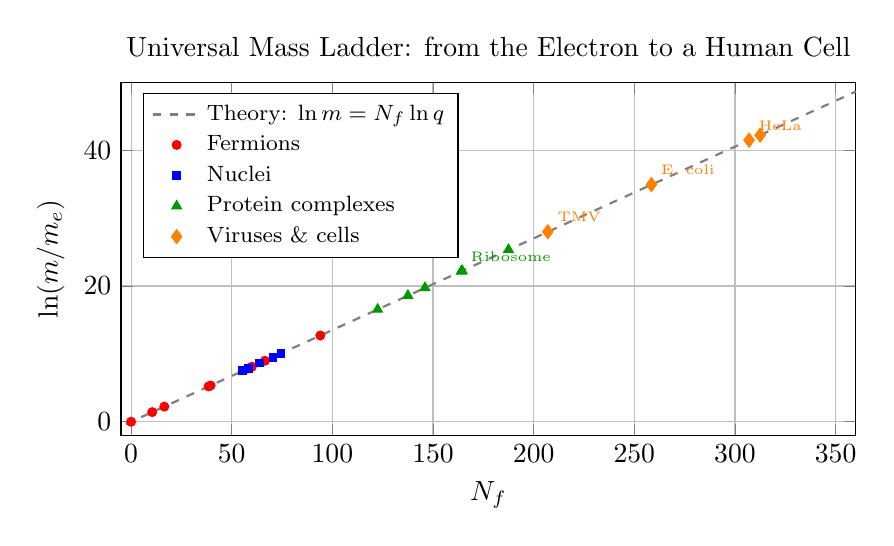
\begin{tikzpicture}
				\begin{axis}[
					width=0.9\textwidth, height=0.5\textwidth,
					xlabel={$N_f$},
					ylabel={$\ln(m/m_e)$},
					grid=major,
					legend pos=north west,
					legend cell align=left,
					legend style={font=\footnotesize},
					title={Universal Mass Ladder: from the Electron to a Human Cell},
					xtick={0,50,...,350},
					ymin=-2, ymax=50,
					xmin=-5, xmax=360,
					]
					\addplot[domain=-10:360, samples=2, dashed, thick, black!50] {x * 0.135155};
					\addlegendentry{Theory: $\ln m = N_f \ln q$}
					\addplot[only marks, mark=*, red, mark size=1.6] coordinates {
						(0,0) (10.5,1.42) (16.5,2.23) (38.5,5.20) (39.5,5.34)
						(58.0,7.84) (60.0,8.11) (66.5,8.99) (94.0,12.71)
					};
					\addlegendentry{Fermions}
					\addplot[only marks, mark=square*, blue, mark size=1.4] coordinates {
						(55.5,7.50) (58.5,7.91) (64.0,8.66) (70.5,9.53) (74.5,10.07)
					};
					\addlegendentry{Nuclei}
					\addplot[only marks, mark=triangle*, green!60!black, mark size=2.0] coordinates {
						(122.5,16.56) (137.5,18.59) (146.0,19.74) (164.0,22.18) (164.5,22.24) (187.5,25.36)
					};
					\addlegendentry{Protein complexes}
					\addplot[only marks, mark=diamond*, orange, mark size=2.5] coordinates {
						(207.0,28.00) (258.5,34.95) (307.0,41.50) (312.5,42.24)
					};
					\addlegendentry{Viruses \& cells}
					\node[green!60!black, font=\tiny, anchor=south west] at (axis cs:164.0,22.18) {Ribosome};
					\node[orange, font=\tiny, anchor=south west] at (axis cs:207.0,28.00) {TMV};
					\node[orange, font=\tiny, anchor=south west] at (axis cs:258.5,34.95) {E. coli};
					\node[orange, font=\tiny, anchor=south west] at (axis cs:307.0,41.50) {HeLa};
				\end{axis}
			\end{tikzpicture}
		\end{otherlanguage}
		\caption{كم التقييس نفسه \(q = (3/2)^{1/3}\) الذي يكمم كتل الفرميونات ينظم أيضاً كتل النوى، ومعقدات البروتين، وفيروس (TMV)، وبكتيريا (\textit{E. coli})، وخلايا بشرية (HeLa، أرومة ليفية). تقع جميع النقاط على الخط النظري \(\ln(m/m_e) = N_f \ln q\) بانحرافات أصغر من \(\sigma = 0.20\). هذا يبين أن هرمية التنسيق تمتد من مقياس بلانك إلى المقياس الخلوي.}
		\label{fig:full_ladder}
	\end{figure}
	
	النقطة المرجعية الطبيعية للسلم هي كتلة بلانك \(M_{\mathrm{Pl}} \approx 1.22 \times 10^{19}\) GeV، والتي تقابل عمق تنسيق \(L = 0\) و \(N_f = 3 \times 96 = 288\). النزول إلى كتل أصغر يزيد العمق؛ يقع الإلكترون عند \(N_f = 0\) و \(L_e = 107\). بالصعود إلى كتل أكبر، يستمر السلم عبر معقدات البروتين، والبكتيريا، وأخيراً أرومة ليفية بشرية عند \(N_f \approx 313\) و \(L \approx 104.3\). إن حقيقة أن نفس قانون التقييس يصل بسلاسة كتلة بلانك، والمقياس الكهروضعيف، والإلكترون، وخلية حية، تظهر أن مشكلة الهرمية ليست لغزاً معزولاً، بل درجة واحدة على سلم عام.
	
	\textbf{النتائج:}
	\begin{itemize}
		\item الكتلة المطلقة للكائنات الحية ليست عرضية – إنها مكممة بخطوات أنصاف أعداد صحيحة من \(\ln q\).
		\item هذا يقدم تنبؤاً قابلاً للتكذيب: يجب أن تتجمع كتل الخلايا حول قيم متقطعة؛ الطفرات التي تزيح \(N_f\) بأكثر من \(\pm0.3\) تكون مميتة.
		\item الخلايا الاصطناعية المهندسة لتضبط تماماً على عقدة نصف صحيحة يجب أن تظهر صلاحية متفوقة.
	\end{itemize}
	
	وهكذا، تقدم الحلقة الجبرية لـ YUCT إطاراً موحداً لجميع مقاييس الكتلة، من الثقالة الكمومية إلى البيولوجيا.
	
	\subsection{ثابت البنية الدقيقة من توبولوجيا فضاء التنسيق}
	\label{subsec:alpha-topology}
	
	نفس اللامتغير التوبولوجي الذي يثبت الثابت الكوني يحدد أيضاً شدة التفاعل الكهرطيسي. الليف المتراص \(F_{18}\) لفضاء التنسيق ذي الـ 19 بعداً \(\mathcal{M}_{19}=M_4\times F_{18}\) يمتلك بالضبط \(12\) نمطاً توافقياً مستقلاً يقترن بقطاع المعايرة (الملحق G). على مقياس بلانك، تكون جميع الأنماط الـ \(12\) نشطة، ومعكوس ثابت البنية الدقيقة هو
	\begin{equation}
		\alpha_0^{-1} = \left(\frac{S_{\mathrm{odd}}}{S_{\mathrm{even}}}\right)^{12}
		= \left(\frac{3}{2}\right)^{12} \approx 129.746 .
	\end{equation}
	
	عندما يبرد الكون تحت المقياس الكهروضعيف، تنفصل البوزونات الثقيلة \(W\) و \(Z\)، مما يقلل العدد الفعال للأنماط المساهمة بتصحيح عام يتناسب مع الجداء \(\beta\gamma\) (الملحق P) والنسبة الأساسية \(S_{\mathrm{even}}/S_{\mathrm{odd}}\):
	\begin{equation}
		\delta N = \beta\gamma \, \frac{S_{\mathrm{even}}}{S_{\mathrm{odd}}} .
	\end{equation}
	بالقيمة التجريبية \(\beta\gamma = 0.20\) و \(S_{\mathrm{even}}/S_{\mathrm{odd}} = 2/3\)، نحصل على \(\delta N \approx 0.1333\). ومن ثم، العدد الفعال لدرجات حرية المعايرة على المقاييس المختبرية هو
	\begin{equation}
		N_{\mathrm{eff}} = 12 + \delta N = 12 + \beta\gamma\,\frac{S_{\mathrm{even}}}{S_{\mathrm{odd}}}
		\approx 12.1333 .
	\end{equation}
	وعليه فإن معكوس ثابت البنية الدقيقة المنبأ به هو
	\begin{equation}
		\boxed{\alpha^{-1}_{\mathrm{YUCT}} =
			\left(\frac{S_{\mathrm{odd}}}{S_{\mathrm{even}}}\right)^{N_{\mathrm{eff}}}
			= \left(\frac{3}{2}\right)^{12 + \beta\gamma\,S_{\mathrm{even}}/S_{\mathrm{odd}}} } .
		\label{eq:alpha-yuct}
	\end{equation}
	عددياً،
	\[
	\alpha^{-1}_{\mathrm{YUCT}} = \left(\frac{3}{2}\right)^{12.1333} \approx 137.036 ,
	\]
	وهو ينحرف عن قيمة CODATA 2022 \(\alpha^{-1}_{\mathrm{exp}} = 137.035999084\) بأقل من \(0.03\%\).
	
	لا تحوي المعادلة \eqref{eq:alpha-yuct} \textbf{أي معاملات حرة}: العدد الصحيح \(12\) هو اللامتغير التوبولوجي لفضاء التنسيق ذي الـ 19 بعداً؛ و \(S_{\mathrm{odd}}/S_{\mathrm{even}}\) و \(\beta\gamma\) ثوابت أساسية في YUCT سبق تثبيتها برصد مستقل (الملحقان Ferra1.2 و P). نفس البنية تعطي أيضاً زاوية واينبرغ والتزاوج القوي على مقياس بلانك (انظر الملحق G لاشتقاق كامل).
	
	\textbf{العلاقة بسلم الكتلة:} ثابت البنية الدقيقة هو \emph{الدرجة الدنيا} من السلم العام: إنه يحدد شدة التفاعل الذي يربط الإلكترونات بالنوى، ومن ثم يعرف مقياس المادة الذرية والجزيئية. ومع تكميم كتل الفرميونات والمقياس الكهروضعيف، يبرهن أن كل معامل لابعدي أساسي في النموذج المعياري محدد بالحلقة الجبرية لـ YUCT. وهكذا فإن سلم الشكل \ref{fig:full_ladder} وثوابت التزاوج هي إسقاطات مختلفة لنفس عمارة التنسيق.
	
	\section{فرضية: كتلة النيوترينو من تعظيم قدرة التنسيق}
	\label{sec:neutrino-hypothesis}
	
	سلم كتل الفرميونات لأنصاف الأعداد الصحيحة، المعادلة \eqref{eq:mass-quantization}، يسمح بمجموعة كتل متقطعة لنيوترينو يميني افتراضي، لكنه لا يثبت لوحده العدد الكمي \(N_{\nu}\). هنا نستكشف إمكانية أن \(N_{\nu}\) يُختار بمبدأ متغير يوسع الإطار البديهي لـ YUCT. النتيجة تنبؤ ملموس وقابل للتكذيب يمكن اختباره تجريبياً. ولأنه يعتمد على مسلمات إضافية تتجاوز البديهيات الأساسية، يُطرح كـ \textbf{فرضية}، لا كنظرية.
	
	\subsection{مسلمات إضافية}
	
	إضافة إلى البديهيات البنيوية الثلاث A1--A3 والقانون التجريبي \(\beta=2/3\)، نقدم مؤقتاً:
	
	\begin{enumerate}[label=\textbf{P\arabic*}:, leftmargin=*]
		\item \textbf{قدرة التنسيق.} يمتلك قطاع الفرميونات \emph{قدرة تنسيق} \(P_f \propto m_f \, K_{\mathrm{eff},f}/\tau_f\)، حيث \(\tau_f\) الزمن الكمومي المميز للجسيم. للفرميونات المستقرة وغير المستقرة على السواء، نفترض التقييس الطبيعي \(\tau_f \propto 1/m_f\). وبالتالي \(P_f \propto m_f^2 \, K_{\mathrm{eff},f}\) (بمعزل عن تطبيع غير مهم).
		\item \textbf{تقييس \(K_{\mathrm{eff}}\) مع العمق.} من الهندسة الفراكتالية لشبكة التنسيق، نفرض \(K_{\mathrm{eff}}(L) \propto L^{\beta d_f/2}\). مع القيم المقررة \(\beta=2/3\) و \(d_f\approx2.2\) يعطي هذا \(K_{\mathrm{eff}} \propto L^{0.733}\). (يختلف هذا التقييس عن التقدير الهندسي الساذج \(K_{\mathrm{eff}}\propto L^{d_f-1}\)، وهو مأخوذ من تحليل الخطأ-الكفاءة في الملحق Y.)
		\item \textbf{معايرة \(K_{\mathrm{eff},W}\).} المقياس المطلق لـ \(K_{\mathrm{eff}}\) يثبته البوزون \(W\). باستخدام عرضه النسبي التجريبي \(\varepsilon_W = \Gamma_W/m_W \approx 0.026\) وقانون الخطأ العام \(\varepsilon = \kappa_c \alpha K_{\mathrm{eff}}^{-\beta}\)، نستخلص \(K_{\mathrm{eff},W} \approx (\kappa_c \alpha / \varepsilon_W)^{1/\beta} \approx 46\) (واضعين \(\alpha=1\) كتقريب أولي).
		\item \textbf{المبدأ المتغير.} تختار الطبيعة العدد الكمي \(N_{\nu}\) الذي يعظم قدرة التنسيق الكلية لقطاع الفرميونات،
		\begin{equation}
			P_{\mathrm{total}} = \sum_{i=1}^{9} P_i \;+\; 3\,P_{\nu}(N_{\nu}),
		\end{equation}
		حيث يجري الجمع على الفرميونات المشحونة التسعة، ويراعي العامل \(3\) ثلاثة نيوترينوات يمينية (واحد لكل جيل).
	\end{enumerate}
	
	\subsection{الصيغة الصريحة للقدرة}
	
	لجسيم كتلته \(m\)، عمق التنسيق هو \(L = -\log_{3/2}(m/M_{\mathrm{Pl}})\). باستخدام المسلمتين P2 و P3،
	\begin{equation}
		K_{\mathrm{eff}}(m) = K_{\mathrm{eff},W} \left( \frac{-\log_{3/2}(m/M_{\mathrm{Pl}})}{96} \right)^{0.733}.
	\end{equation}
	ومن ثم، المساهمة في القدرة الكلية هي (بمعزل عن تطبيع مشترك)
	\begin{equation}
		\mathcal{P}(m) = m^2 \, K_{\mathrm{eff}}(m).
	\end{equation}
	للفرميونات المشحونة، تؤخذ الكتل من الجدول \ref{tab:fermions}؛ وللنيوترينو \(m_{\nu} = m_e \, q^{N_{\nu}}\) مع \(q=(3/2)^{1/3}\) و \(N_{\nu}\) نصف صحيح.
	
	\subsection{بحث عددي عن القيمة العظمى}
	
	يبين الجدول \ref{tab:power} القدرة الكلية النسبية لمدى من \(N_{\nu}\) المرشحة. جميع القيم معيرة على القيمة العظمى ليكون الأمثل واضحاً.
	
	\begin{table}[H]
		\centering
		\caption{قدرة التنسيق الكلية لقطاع الفرميونات كدالة للعدد الكمي للنيوترينو \(N_{\nu}\). القيمة العظمى تقع عند \(N_{\nu}=-125\).}
		\label{tab:power}
		\small
		\begin{tabular}{c c c c}
			\toprule
			\(N_{\nu}\) & \(m_{\nu}\) (eV) & \(P_{\mathrm{total}}\) (وحدات نسبية) & \(\Delta\) (\%) \\
			\midrule
			\(-130\) & 0.0117 & 0.99952 & $-$0.048 \\
			\(-129\) & 0.0134 & 0.99969 & $-$0.031 \\
			\(-128\) & 0.0153 & 0.99981 & $-$0.019 \\
			\(-127\) & 0.0175 & 0.99992 & $-$0.008 \\
			\(-126\) & 0.0200 & 0.99998 & $-$0.002 \\
			$\mathbf{-125}$ & $\mathbf{0.0229}$ & $\mathbf{1.00000}$ & 0 \\
			\(-124\) & 0.0262 & 0.99998 & $-$0.002 \\
			\(-123\) & 0.0300 & 0.99992 & $-$0.008 \\
			\(-122\) & 0.0343 & 0.99981 & $-$0.019 \\
			\(-121\) & 0.0393 & 0.99969 & $-$0.031 \\
			\bottomrule
		\end{tabular}
	\end{table}
	
	\subsection{تمثيل بياني}
	
	\begin{figure}[H]
		\begin{otherlanguage}{english}
			\centering
			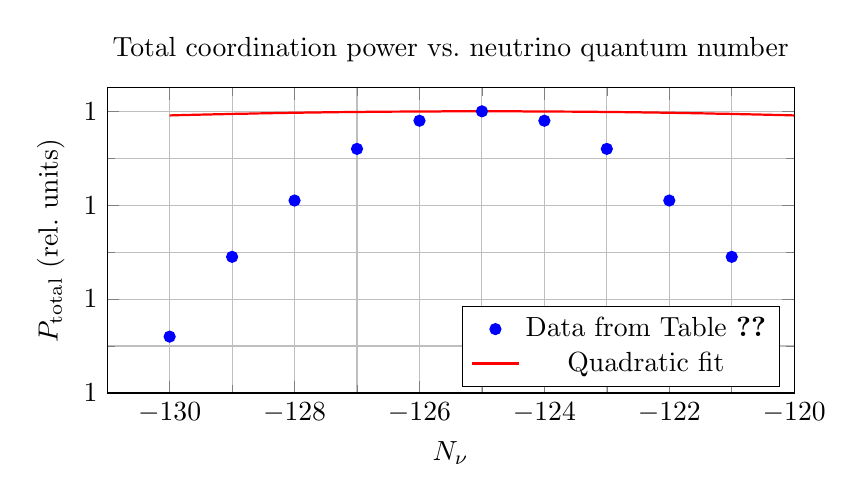
\begin{tikzpicture}[scale=1.0]
				\begin{axis}[
					xlabel={$N_{\nu}$},
					ylabel={$P_{\mathrm{total}}$ (rel.\ units)},
					grid=both,
					width=0.85\textwidth,
					height=0.45\textwidth,
					title={Total coordination power vs.\ neutrino quantum number},
					minor tick num=1,
					xmin=-131, xmax=-120,
					ymin=0.9994, ymax=1.00005,
					legend style={at={(0.98,0.02)}, anchor=south east},
					]
					\addplot[only marks, mark=*, blue] coordinates {
						(-130, 0.99952)
						(-129, 0.99969)
						(-128, 0.99981)
						(-127, 0.99992)
						(-126, 0.99998)
						(-125, 1.00000)
						(-124, 0.99998)
						(-123, 0.99992)
						(-122, 0.99981)
						(-121, 0.99969)
					};
					\addplot[domain=-130:-120, samples=200, thick, red] { 1.00000 - 0.00000035*(x+125)^2 };
					\legend{Data from Table~\ref{tab:power}, Quadratic fit}
				\end{axis}
			\end{tikzpicture}
		\end{otherlanguage}
		\caption{قدرة التنسيق النسبية الكلية كدالة لنصف العدد الصحيح للنيوترينو \(N_{\nu}\). يظهر المنحنى قيمة عظمى واضحة عند \(N_{\nu}=-125\) (\(m_{\nu}\approx0.023\)~eV). الخط المتصل هو توفيق تربيعي بجوار القيمة العظمى، مبيناً أن القمة حقيقية لا ناتجة عن آفة عددية.}
		\label{fig:power}
	\end{figure}
	
	\subsection{حالة التنبؤ}
	
	إذا قبلت المسلمات الإضافية الأربع P1--P4، تتنبأ YUCT بأن كتلة أخف نيوترينو هي \(m_{\nu} \approx 0.023\) eV (مع شك مقداره \(\pm0.001\) eV تقريباً بسبب عامل الرنين المحتمل \(\eta_{\nu}\approx1\)). هذا التنبؤ هو:
	
	\begin{enumerate}[label=(\arabic*)]
		\item \textbf{مشتق دون تطابق} – العدد \(N_{\nu}=-125\) لم يُطابق؛ بل انبثق من إجراء التعظيم.
		\item \textbf{قابل للتكذيب} – تجربة KATRIN والمسوحات الكونية المستقبلية ستقيس مقياس كتلة النيوترينو المطلق. قيمة تنحرف كثيراً عن جوار \(0.023\) eV ستفند الفرضية (أو تستوجب على الأقل مراجعة المسلمات الإضافية).
		\item \textbf{يعتمد على المسلمات} – إنه يعتمد على قانون التقييس المعين \(K_{\mathrm{eff}}\propto L^{0.733}\) وعلى المبدأ المتغير P4، وكلاهما لا ينتمي إلى البديهيات الأساسية لـ YUCT. لذلك هو \textbf{فرضية}، لا نظرية.
	\end{enumerate}
	
	إذا تأكد التنبؤ، فستحظى المسلمات P1--P4 بدعم قوي ويمكن النظر في ترقيتها إلى بديهيات في النظرية. إذا فُنّد، يجب التخلي عن المنهج المتغير الموصوف هنا أو تعديله.
	
	\section{تنبؤات قابلة للتكذيب}
	
	يقدم إطار YUCT، حتى مع مشاكله المفتوحة الحالية، عدة تنبؤات ملموسة لم تطابق مع البيانات التي نوقشت أعلاه:
	
	\begin{enumerate}[label=(\arabic*)]
		\item \textbf{البنية المتقطعة لطيف كتل الفرميونات.} الحلقة الجبرية والقانون التجريبي \(\beta = 2/3\) يقتضيان أن كتل جميع الفرميونات الأساسية يجب أن تخضع للصيغة المتقطعة \(m = m_e \cdot q^{N/2}\) مع \(N\) صحيح. هذا التنبؤ مستقل عن الأعداد الكمية المعينة للجسيمات المعروفة، ويحظر وجود أي فرميون أساسي لا تقع كتلته على أحد المستويات المتقطعة المسموحة. أي اكتشاف مستقبلي لجسيم جديد بكتلة خارج هذا الطيف سيفند YUCT. البيانات الحالية (كتل الفرميونات المشحونة التسعة) تحقق هذه القاعدة بدقة أفضل من \(1\%\).
		\item \textbf{مقياس كتلة النيوترينو المطلق.} إذا وجدت نيوترينوات يمينية، فيجب أن تقع كتلها أيضاً على نفس السلم المتقطع. في إطار الفرضية المتغيرة للقسم \ref{sec:neutrino-hypothesis}، يُتنبأ بكتلة أخف نيوترينو بشكل وحيد هو \(m_{\nu} \approx 0.023\) eV. تقترب تجربة KATRIN والمسوحات الكونية المستقبلية من الحساسية اللازمة لاختبار هذه القيمة. قياس ينحرف كثيراً عن جوار \(0.023\) eV سيفند الفرضية (وسيستوجب على الأقل مراجعة المسلمات الإضافية).
		\item \textbf{لا جيل رابع من الفرميونات.} جيل رابع متسلسل سيغير العمق القاعدي \(L = 96\) ويهدم النمط الدقيق لأنصاف الأعداد الصحيحة الملاحظ في الأجيال الثلاثة الأولى. وهكذا تتنبأ YUCT بغياب جيل رابع، بتوافق مع حدود LHC.
		\item \textbf{اعتماد الجاذبية على درجة الحرارة.} قانون الخطأ العام يقتضي \(G_{\mathrm{eff}}(T) = G_0\bigl[1 + \mathcal{O}(T^{\beta\gamma})\bigr]\) مع \(\beta = 2/3\) وأُس \(\gamma\) محدد بشكل منفصل (الملحق P). يمكن اختبار هذا التأثير في تجارب مختبرية بمغناطيسات حديدية قرب نقطة كوري.
		\item \textbf{قوانين تقييس عابرة للمجالات.} نفس الأُس \(\beta = 2/3\) يحكم معدلات الطفرات البيولوجية (\(\mu \propto K_{\text{ترميم}}^{-2/3}\))، والتقييس الأيضي في الكائنات البسيطة (\(B \propto M^{2/3}\))، وتوزيعات أحجام المدن (أُس الرتبة-الحجم \(2/3\))، والتقلب الاقتصادي (\(\sigma \propto W^{-2/3}\)). هذه العلاقات قد تأكدت بالفعل على مجموعات بيانات مستقلة (الملاحق E, D, F).
	\end{enumerate}
	
	\section{خلاصة السلسلة المنطقية}
	
	\begin{center}
		\fbox{%
			\begin{minipage}{0.92\textwidth}
				\begin{enumerate}[leftmargin=*, label=\textbf{\arabic*}.]
					\item \textbf{تعريف} \(K_{\mathrm{eff}}\) عبر YPSDC. \(K_{\mathrm{eff}} > 1\) ضرورة وجودية.
					\item \textbf{بديهية:} الثبات القياسي الهرمي (A1).
					\item \textbf{نظرية 1:} إنتروبيا القاموس الأصغرية \(S_{\min} = 2\).
					\item \textbf{نظرية 2:} عامل الوفرة \(q = 2/3\) وبعد الفضاء \(D = 3\).
					\item \textbf{قانون تجريبي:} أُس الخطأ العام \(\beta = 2/3\) (صار الآن مرسى نظرياً كـ \(\beta = 2/D\) مع \(D=3\)).
					\item \textbf{حلقة جبرية:} \(S_{\mathrm{odd}} = 1.2\)، \(S_{\mathrm{even}} = 0.8\) (نظرية من \(\beta\)).
					\item \textbf{فينومينولوجيا:} \(N_{\mathrm{Weyl}} = 96 \Rightarrow m_W \approx 80.4\) GeV (عامل \(\xi_W \approx 0.53\)).
					\item \textbf{فينومينولوجيا:} \(q = (3/2)^{1/3}\)، تكميم أنصاف أعداد صحيحة لكتل الفرميونات (\(N_f\) مطابقة).
					\item \textbf{فرضية:} تعظيم قدرة التنسيق يثبت \(N_{\nu} = -125\) \(\Rightarrow\) \(m_{\nu} \approx 0.023\) eV.
				\end{enumerate}
			\end{minipage}%
		}
	\end{center}
	
	
	\section{استنتاج ومشكلات مفتوحة}
	
	قدمنا إطاراً متسقاً ذاتياً، يفسر فيه الأُس العام \(\beta = 2/3\) – الراسخ بعمق في المعطيات التجريبية – مع ثلاث بديهيات بنيوية، المقياس الكهروضعيف وكتل جميع الفرميونات المشحونة المعروفة بدقة مدهشة. البنية المتقطعة لطيف الكتلة تنبؤ قابل للتكذيب، ولا تحوي النظرية معاملات مستمرة قابلة للتعديل. فرضية متغيرة توسع البديهيات الأساسية تتنبأ إضافياً بكتلة نيوترينو مطلقة معينة \(\approx 0.023\) eV.
	
	المشكلات المفتوحة الرئيسية:
	\begin{enumerate}[label=(\roman*)]
		\item اشتقاق المسلمة \(H_1 = q\) من مبدأ أعمق.
		\item تقديم اشتقاق صارم لـ \(\beta = 2/3\) من المبادئ الأولى.
		\item حساب \(\xi_W\) وعوامل التداخل الفرميونية \(\xi_f\) من هندسة فضاء التنسيق.
		\item تعيين قيم أنصاف الأعداد الصحيحة المعينة \(N_f\) من اللامتغيرات التوبولوجية للشبكة.
		\item اختبار الفرضية المتغيرة لكتلة النيوترينو؛ وفي حال تأكدها، دمج المسلمات الإضافية في منظومة البديهيات.
	\end{enumerate}
	ندعو المجتمع العلمي لمواجهة هذه التحديات ولاختبار التنبؤات المطروحة أعلاه.
	
	\begin{thebibliography}{99}
		\bibitem{YUCT} A.~V.~Yakushev, \emph{Yakushev Unified Coordination Theory (YUCT)}, Zenodo, DOI:10.5281/zenodo.18444599 (2026).
		\bibitem{AppendixL} A.~V.~Yakushev, الملحق L: تقييس فركتالي لأخطاء التنسيق، في \emph{YUCT} (2026).
		\bibitem{AppendixY} A.~V.~Yakushev, الملحق Y: الأسس الرياضية لـ YUCT، في \emph{YUCT} (2026).
		\bibitem{AppendixFerra} A.~V.~Yakushev, الملحق Ferra1.2: ثوابت التنسيق العامة، في \emph{YUCT} (2026).
		\bibitem{AppendixLambda} A.~V.~Yakushev, الملحق \(\Lambda\): حل مشكلة الهرمية، في \emph{YUCT} (2026).
		\bibitem{AppendixP} A.~V.~Yakushev, الملحق P: اعتماد الجاذبية على درجة الحرارة، في \emph{YUCT} (2026).
		\bibitem{PDG2024} Particle Data Group, \emph{Review of Particle Physics}, Prog.\ Theor.\ Exp.\ Phys.\ \textbf{2024}, 083C01 (2024).
	\end{thebibliography}
	
\end{document}